\section{Durchführung}
\label{sec:Durchfuehrung}
In diesem Kapitel sollen die einzelnen Schritte des Versuches erklärt werden.
Alle Schaltungen werden auf einem Steckbrett, Breadboard oder Steckplatine genannten Konstrukt
aufgebaut. Das vermeidet aufwändiges Löten von Lochrasterplatinen.


\subsection{Der invertierende Linearverstärker}
Für zwei verschiedene Widerstandsverhältnisse wird die Frequenzabhängigkeit 
des Verstärkungsfaktors sowie der Phasenverschiebung untersucht. Dazu werden ein- 
und Ausgansspannung der Schaltung gemessen und am Oszilloskop die Phasenverschiebung abgelesen.
Die Schaltung wird wie in \autoref{fig:SPlinearverstaerker} zu sehen aufgebaut.
\begin{figure}
    \centering
    
\includegraphics[width=1\textwidth]{content/grafiken/SPlinearverstaerker.PNG}
    \caption{Schaltplan des invertierenden Linearverstärkers. }
    \label{fig:SPlinearverstaerker}
  \end{figure}



\subsection{Der Umkehrintegrator und der invertierender Differenzierer}
Für diese beiden Teilversuche werden Schaltungen nach \autoref{fig:SPumkehrintegrator} und 
\autoref{fig:SPumkehrdifferenzierer} auf das Steckbrett gesteckt.
Bei diesen beiden Schaltungen wird das verhalten bei verschiedenen Einganssignalformen untersucht.
Dazu wird von einem Signalgenerator zunächst ein Sinussignal, dann eine Rechteckspannung und anschließend
eine Dreiecksspannung erzeugt und diese als Einganssignal für die jeweilige Schaltung genutzt.
Auf eienm Oszilloskop wird dann das Ausgangsignal dargestellt.
Zudem wird auch hier das Frequenzverhalten des Verstärkungsfaktors untersucht.
\begin{figure}
    \centering
    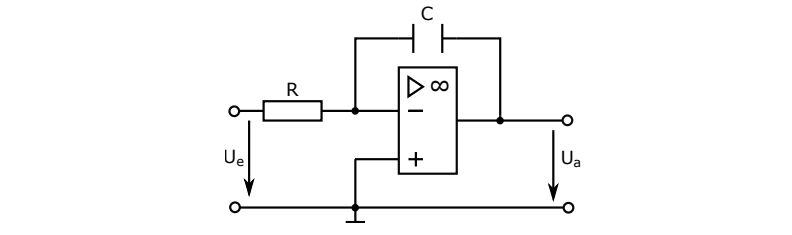
\includegraphics[width=1\textwidth]{content/grafiken/SPumkehrintegrator.PNG}
    \caption{Schaltplan des Umkehrintegrators.}
    \label{fig:SPumkehrintegrator}
  \end{figure}

  \begin{figure}
    \centering
    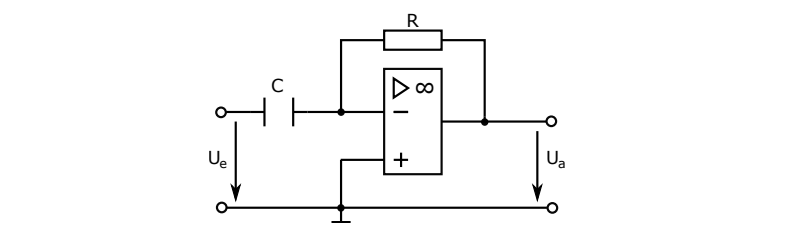
\includegraphics[width=1\textwidth]{content/grafiken/SPumkehrdifferenzierer.PNG}
    \caption{Schaltplan des invertierenden Differenzierers.}
    \label{fig:SPumkehrdifferenzierer}
  \end{figure}



\subsection{Der Schmitt-Trigger}
Für die Untersuchung des Schmitttriggers wird der Operationsverstärker nach \autoref{fig:SPschmitttrigger}
als Schwellwertschalter beschaltet. Durch almähliches erhöhen der Amplitude des eingespeisten Snussignals 
wird durch gleichzeitige Spannungsmessung der Kippunkt ermittelt an welchem der Trigger durchschaltet und 
sperrt.
\begin{figure}
    \centering
    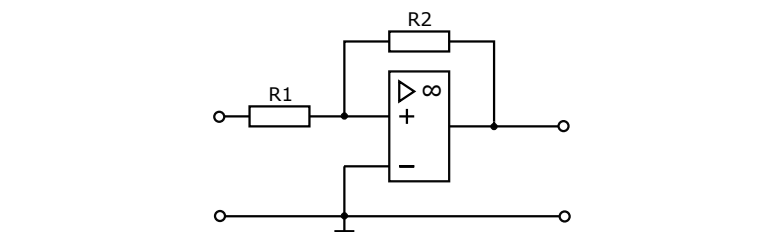
\includegraphics[width=1\textwidth]{content/grafiken/SPschmitttrigger.PNG}
    \caption{Schaltplan des Schmitt-Triggers.}
    \label{fig:SPschmitttrigger}
  \end{figure}




\subsection{Der Signalgenerator}
Beim Signalgenerator wederden Schmitttrigger und Umkehrintegrator hintereinander geschaltet und 
die Signalformen werden genauer untersucht. Die Schaltung wird hier nach \autoref{fig:SPsignalgenerator}
aufgebaut.

\begin{figure}
    \centering
    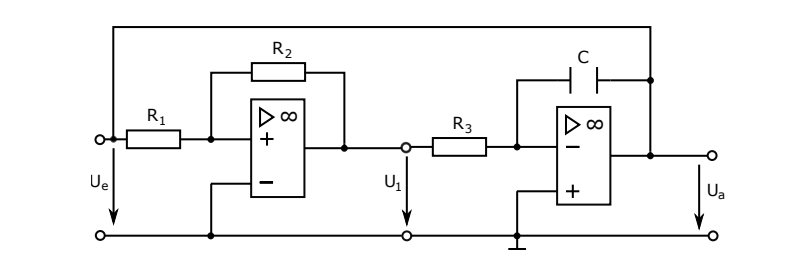
\includegraphics[width=1\textwidth]{content/grafiken/SPsignalgenerator.PNG}
    \caption{Schaltplan des Signalgenerators.}
    \label{fig:SPsignalgenerator}
  \end{figure}